\documentclass[10pt]{article}
\usepackage[spanish,activeacute]{babel}
\usepackage{graphicx}
\usepackage[margin=3cm]{geometry}
\title{\bfseries\Huge Puzlive 1.0\\ Manual de Uso}
\author{Leonardo Tamayo \\Pedro Iñiguez \\Carlos Caicedo}
\date{}
\begin{document}
\begin{minipage}{0.65\textwidth}
\begingroup
\let\center\flushleft
\let\endcenter\endflushleft
\maketitle

\endgroup
\end{minipage}
\begin{minipage}{0.3\textwidth}

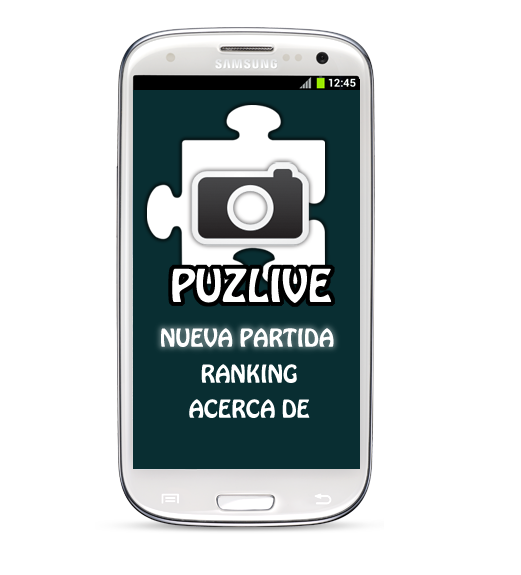
\includegraphics[height=7cm,width=6cm]{androidpro4.png}
\end{minipage}

\section{Resumen}
	Este Manual es una pequeña y util guia para el usuario de la App PuzLive. Le brindara informacion importante acerca de la aplicacion y le enseñara como 
utilizarla y la variedad de opciones que posee. Gracias a este manual, el usuario sera capaz de recorrer la aplicacion sin ningun problema y entretenerse al usarla.

\section{Comandos}
	Las teclas que le ser\'an de utilidad durante la aplicaci\'on:
	\\1.- Return : El bot\'on RETURN propio del celular, permite regresar a las ventanas anteriores de la aplicaci\'on
	\\2.- Home : El bot\'on HOME propio del dispositivo permite desplegar un menu dentro de la actividad de armar el rompecabezas para mostrar el bot\'on REFRESH
	en el modo EST\'ATICO o el bot\'on HINT en el modo din\'amico.
	

\section{Ejecutando la Aplicacion}
	\subsection{Instalando la Aplicacion}
		Para instalar nuestra aplicacion, debemos copiar el archivo PuzLive.apk a nuestro telefono celular desde nuestra computadora a traves de un cable USB 
		y correrlo a travez de la App "apk installer". Una vez hecho esto, nuestra App estara instalada en nuestro telefono.
	\subsection{Seleccionando la Aplicacion} 
		Una vez que la aplicacion este instalada, encontraremos nuestra aplicacion asi: \\
		\begin{center}
		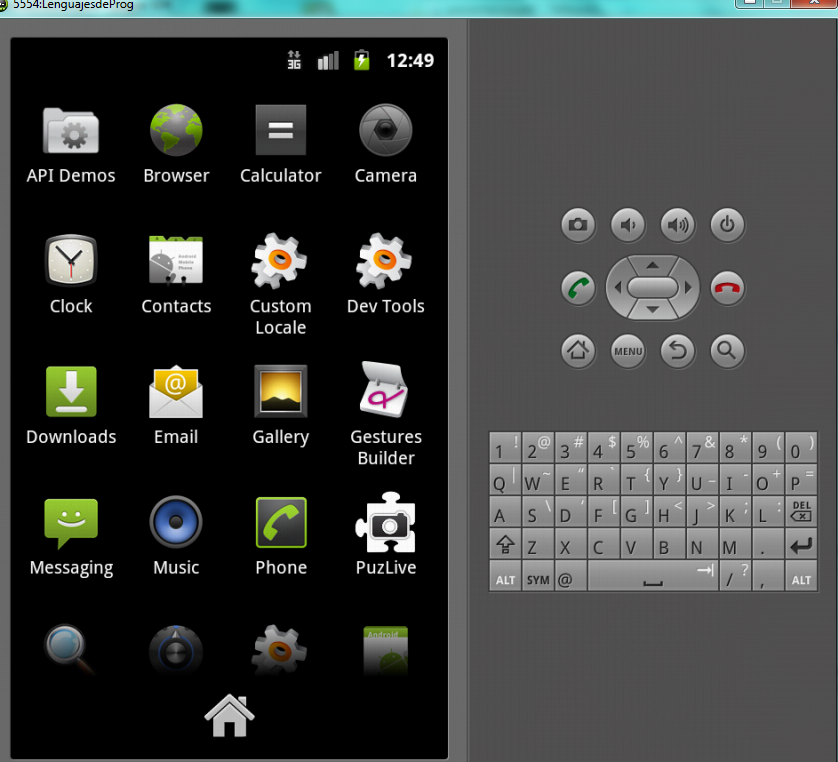
\includegraphics[height=8cm,width=10cm]{outmenu.png}
		\end{center}	
		 Solo le damos un TOUCH (toque) al icono de PuzLive y asi iniciamos la App.	

\section{Recorriendo PuzLive}
	Al dar click al icono de PuzLive, se nos habilita el siguiente menu:
	\begin{center}
		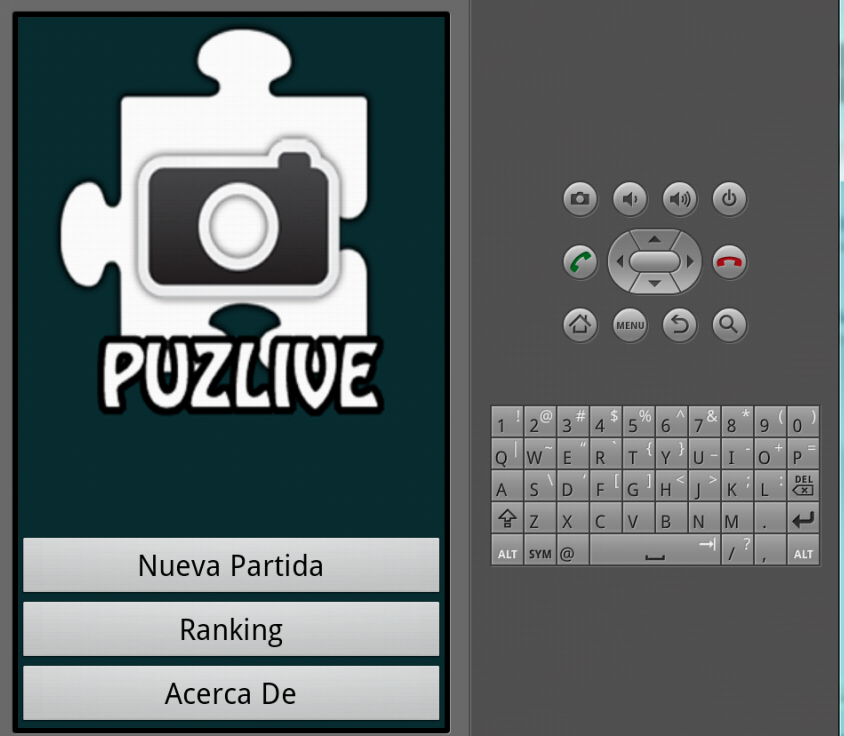
\includegraphics[height=8cm,width=10cm]{menuPrin.png}
	\end{center}	
	
	\subsection{Acerca De}
		Esta opcion mostrara en pantalla la informacion con respecto a la aplicacion:
		\begin{center}
		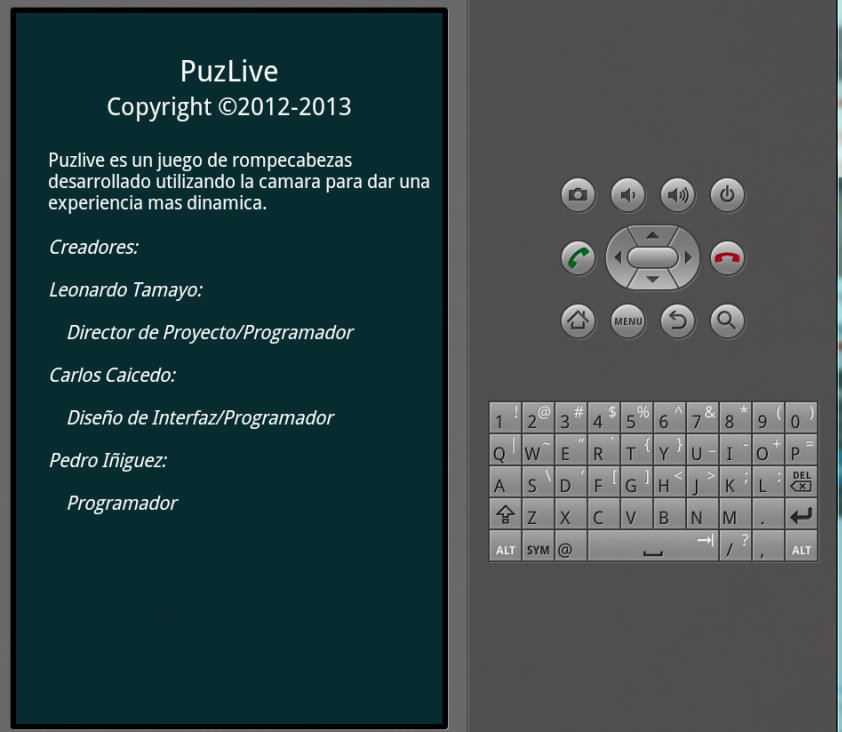
\includegraphics[height=8cm,width=10cm]{acerca.png}
		\end{center}	
		
	\subsection{Ranking}
		Esta opcion mostrar\'a los puntajes de acuerdo al tiempo en orden descendente de los jugadores que hayan registrado su puntaje en la aplicacion

	\subsection{Nueva Partida}
		Existen dos tipos de juego con sus respectivas dificultades con los cuales el Usuario podra disfrutar de la aplicacion:
		\begin{center}
		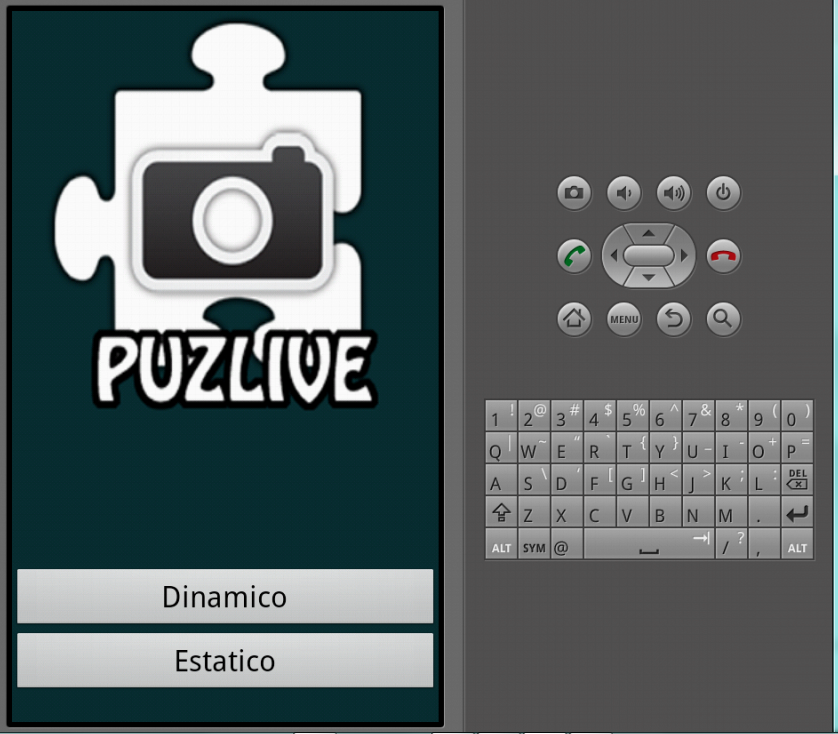
\includegraphics[height=8cm,width=10cm]{dosgame.png}
		\end{center}	
\section{Interface de Juego}
	Al haber elejido uno de los dos modos de juego, la siguiente ventana de niveles se despliega:
		\begin{center}
		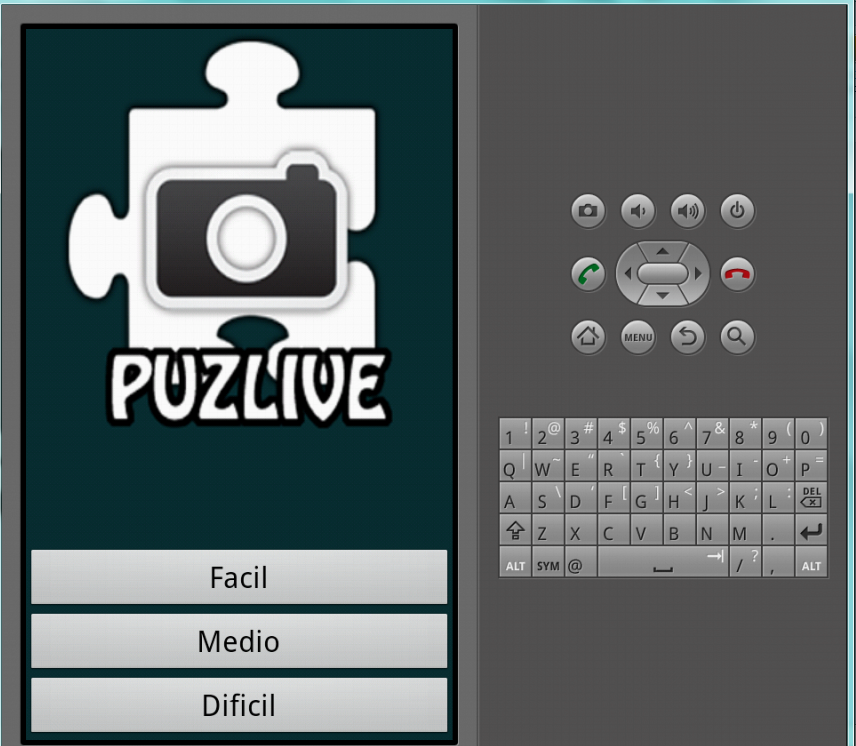
\includegraphics[height=8cm,width=10cm]{niveles.png}
		\end{center}	
	La dificultad se basa en la cantidad de piezas que poseera el rompecabezas. La cantidad de piezas para cada nivel son las siguientes:
	\\ Facil   - 20 Piezas
	\\Medio - 45 Piezas
	\\Dificil  - 55 Piezas
	\\La imagen estara partida en la cantidad de piezas indicada. Usted debe intercambiar las celdas de imagenes entre ellas hasta poder formar el paisaje real que esta observando el dispositivo.
	\\ ¿Como intercambio las celdas?
	\\ - Es sencillo intercambiar las celdas, usted solo debe tocar una de ellas y luego tocar la otra con la cual desea que se cambie. Usted observara como estas celdas cambian entre ellas.
	\\ ¿Cuales o que son las celdas?
	\\ - Las celdas son las piezas del rompecabezas, cada uno de los rectangulos mezclados de la imagen real.
	\\Una vez seleccionado el nivel, se iniciar\'a la camara y se la mostrara en la pantalla del telefono m\'ovil.
	Para usted poder comenzar a armar el rompecabezas, necesitara primero revolver las piezas de este; para ello usted debe agitar el celular y automaticamente las piezas se mezclaran en celdas 
	en toda la plantalla.
	\begin{center}
	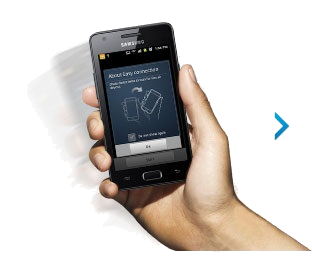
\includegraphics[height=8cm,width=10cm]{shake.png}
	\end{center}	
	\begin{center}
	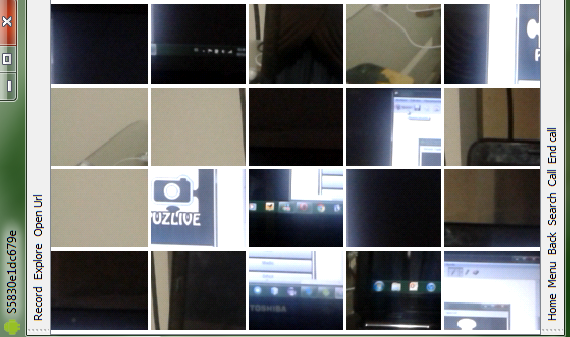
\includegraphics[height=8cm,width=10cm]{inter.png}
	\end{center}	
	\subsection{Est\'atico}
		El modo est\'atico consiste en mostrar una imagen inicial del video e ir armando el rompecabezas en base a ella. 
	\\¿Cual es lo diferente de un puzzle normal?
	\\ - Existe el bot\'on REFRESH el cual cambia la imagen que se tomo en un momento, por la actual que vio la camara al momento de aplastar el bot\'on. 
	\begin{center}
	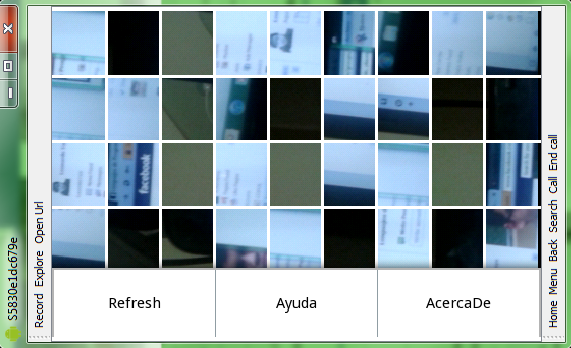
\includegraphics[height=7cm,width=10cm]{refresh.png}
	\end{center}	
	\subsection{Din\'amico}
		El modo din\'amico le permite armar el rompecabezas mientras se le muestra la imagen partida de lo que observa la camara. En otras palabras
		usted tendra que armar un rompecabezas mientras cambia la imagen para completar.
	\\Ademas, existe el bot\'on HINT que le permite obtener ayuda de la aplicaci\'on, de tal manera que una pieza aleatoria se coloque en su posici\'on real.
	\begin{center}
	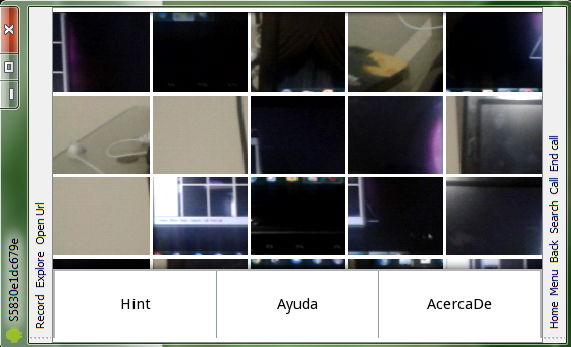
\includegraphics[height=7cm,width=10cm]{hint.png}
	\end{center}	
\section{Final del Juego}
	Usted habr\'a completado el juego cuando la imagen que muestra la aplicacion sea la real. En ese momento se mostrara un mensaje con su puntuaci\'on y el juego habr\'a finalizado.
	\begin{center}
	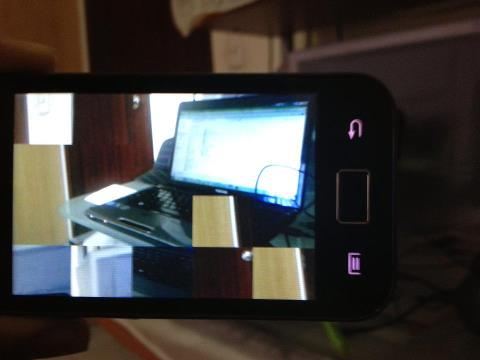
\includegraphics[height=7cm,width=10cm]{completando.jpg}
	\end{center}	
	\begin{center}
	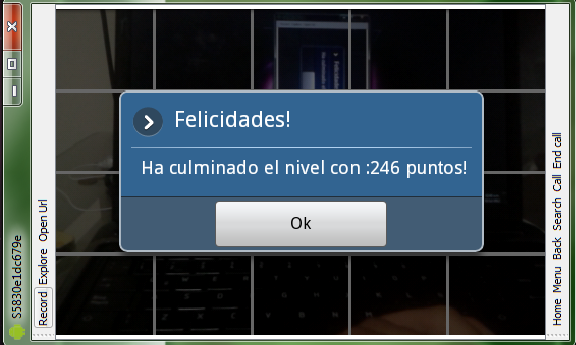
\includegraphics[height=7cm,width=10cm]{gano.png}
	\end{center}	
		


\end{document}